\documentclass{report}
\usepackage{lmodern}
\author{Andreas Schachner}
\title{Dokumentation zum Uni-Heidelberg-App-Projekt}
\usepackage[top=3cm, bottom=3cm, inner=3.5cm, outer=3cm]{geometry}
\usepackage[T1]{fontenc}
\usepackage{amssymb}
\usepackage{pifont} 
\usepackage{longtable} 
\usepackage{tabularx} 
\usepackage{graphicx} 
\usepackage{amsmath}
\usepackage[ngerman]{babel} 
\usepackage[automark,headsepline,plainheadsepline]{scrpage2}
\usepackage{endnotes}
\usepackage{csquotes}
\usepackage{hyperref}
\hypersetup{colorlinks=true,urlcolor=blue,linkcolor=blue}
\usepackage{relsize}
\usepackage{xcolor}
\usepackage{soul}
\usepackage{endnotes}
\setcounter{tocdepth}{2}
\pagestyle{scrheadings}
\ihead[\rightmark]{\rightmark}{}
%\renewcommand*\thechapter{\arabic{chapter}}
%\pagestyle{headings}
%\chead[\pagemark]{{\thechapter} - \chaptername}
\usepackage{pst-all}
\usepackage{blindtext}
\usepackage{fontspec}
\newfontfamily{\codefont}{Menlo}

\usepackage{color,xcolor}
\definecolor{nsclass}{RGB}{124,32,176}
\definecolor{atnotation}{RGB}{204,0,164}
\definecolor{import}{RGB}{128,70,30}
\definecolor{comment}{RGB}{0,140,0}
\definecolor{string}{RGB}{229,0,0}
\definecolor{method}{RGB}{70,0,134}
\definecolor{class}{RGB}{59,131,138}
\definecolor{custommethod}{RGB}{32,90,95}
\definecolor{number}{RGB}{56,0,225}
\definecolor{customgray}{RGB}{211,211,211}
\definecolor{highlight}{RGB}{255,243,153}

\usepackage{listings}
\lstloadlanguages{[Objective]C,bash}
\lstset{language=[Objective]C,tabsize=4, keepspaces=false,
    xleftmargin=0em,xrightmargin=-1em, aboveskip=1em, % Margin adjustment
    %backgroundcolor=\color{customgray},    % Background color (Default:gray)
    frame=none,                            % Frame not needed
    breakindent=22pt,
    numbers=left,stepnumber=1,numberstyle=\tiny\color{black}\codefont,
    basicstyle=\fontsize{9pt}{1em}\selectfont\codefont,
    commentstyle=\fontsize{9pt}{0.75em}\selectfont\codefont\color{comment},
    showspaces=false,
    showstringspaces=false,
    flexiblecolumns=true,
    breaklines=true, breakautoindent=true,breakindent=4em,
    escapeinside={/*@}{@*/},
    morecomment=[s][\color{string}]{@"}{"},
    morecomment=[l][\color{import}]{\#},
    morecomment=**[s][\color{nsclass}]{NS}{];},
    morecomment=**[s][\color{nsclass}]{UI}{];},
    morecomment=**[s][\color{nsclass}]{NS}{(},
    morecomment=**[s][\color{nsclass}]{UI}{)},
    morecomment=**[s][\color{nsclass}]{UI}{*},
    morecomment=**[s][\color{nsclass}]{NS}{*},
    morecomment=*[s][\color{nsclass}]{UI}{\ },
    morecomment=*[s][\color{nsclass}]{NS}{\ },
    literate= {Ö}{{\"O}}1 {Ä}{{\"A}}1 {Ü}{{\"U}}1 {ß}{{\ss}}2 {ü}{{\"u}}1
 {ä}{{\"a}}1 {ö}{{\"o}}1,
}
\lstset{emph=[1]{  % <--Add your own Class Names before the percentage mark
       },emphstyle=[1]{\color{class}},
       moreemph=[5]{ % <--Add your own Method Names before the percentage mark
       },emphstyle=[5]{\color{method}},
}
\lstset{
    emph=[3]{@implementation, @synthesize, @interface, @property, @dynamic,
    @end, @protocol, @class, @selector, break, case, catch, class, copy, const, __finally, __exception,
    __try, const_cast, continue, private, public, protected, __declspec,
    default, delete, deprecated, dllexport, dllimport, do, dynamic_cast, else,
    enum, explicit, extern, if, for, friend, getter, goto, inline, mutable,
    naked, namespace, new, nil, NO, noinline, nonatomic, noreturn, nothrow,
    NULL, readonly, readwrite, register, reinterpret_cast, retain, return,
    SEL, selectany, self, setter, sizeof, static, static_cast, strong, struct, super,
    switch, template, thread, throw, true, false, try, typedef, typeid,
    typename, union, using, uuid, virtual, void, volatile, weak, whcar_t, while, YES,
    ATOM, BOOL, BOOLEAN, BYTE, CHAR, COLORREF, DWORD, DWORDLONG, DWORD_PTR,
    DWORD32,DWORD64, FLOAT, HACCEL, HALF_PTR, HANDLE, HBITMAP, HBRUSH,
    HCOLORSPACE, HCONV, HCONVLIST, HCURSOR, HDC, HDDEDATA, HDESK, HDROP,
    HDWP, HENHMETAFILE, HFILE, HFONT, HGDIOBJ, HGLOBAL, HHOOK, HICON,
    HINSTANCE, HKEY, HKL, HLOCAL, HMENU, HMETAFILE, HMODULE, HMONITOR,
    HPALETTE, HPEN, HRESULT, HRGN, HRSRC, HSZ, HWINSTA, HWND, INT, INT_PTR,
    INT32, INT64, LANGID, LCID, LCTYPE, LGRPID, LONG, LONGLONG, LONG_PTR,
    LONG32, LONG64, LPARAM, LPBOOL, LPBYTE, LPCOLORREF, LPCSTR, LPCTSTR,
    LPCVOID, LPCWSTR, LPDWORD, LPHANDLE, LPINT, LPLONG, LPSTR, LPTSTR, LPVOID,
    LPWORD, LPWSTR, LRESULT, PBOOL, PBOOLEAN, PBYTE, PCHAR, PCSTR, PCTSTR,
    PCWSTR, PDWORDLONG, PDWORD_PTR, PDWORD32, PDWORD64, PFLOAT, PHALF_PTR,
    PHANDLE, PHKEY, PINT, PINT_PTR, PINT32, PINT64, PLCID, PLONG, PLONGLONG,
    PLONG_PTR, PLONG32, PLONG64, POINTER_32, POINTER_64, PSHORT, PSIZE_T,
    PSSIZE_T, PSTR, PTBYTE, PTCHAR, PTSTR, PUCHAR, PUHALF_PTR, PUINT, PUINT_PTR,
    PUINT32, PUINT64, PULONG, PULONGLONG, PULONG_PTR, PULONG32, PULONG64, PUSHORT,
    PVOID, PWCHAR, PWORD, PWSTR, SC_HANDLE, SC_LOCK, SERVICE_STATUS_HANDLE,
    SHORT, SIZE_T, SSIZE_T, TBYTE, TCHAR, UCHAR, UHALF_PTR, UINT, UINT_PTR,
    UINT32, UINT64, ULONG, ULONGLONG, ULONG_PTR, ULONG32, ULONG64, USHORT,
    USN, VOID, WCHAR, WORD, WPARAM, WPARAM, WPARAM, char, bool, short, int, uint,
    __int32, __int64, __int8, __int16, long, float, double, __wchar_t, clock_t,
    _complex, _dev_t, _diskfree_t, div_t, ldiv_t, _exception, _EXCEPTION_POINTERS,
    FILE, _finddata_t, _finddatai64_t, _wfinddata_t, _wfinddatai64_t,
        __finddata64_t,
    __wfinddata64_t, _FPIEEE_RECORD, fpos_t, _HEAPINFO, _HFILE, lconv, intptr_t,
    id, jmp_buf, mbstate_t, _off_t, _onexit_t, _PNH, ptrdiff_t,
    _purecall_handler, sig_atomic_t, size_t, _stat, __stat64, _stati64,
    terminate_function, time_t, __time64_t, _timeb, __timeb64, tm, uintptr_t,
    _utimbuf, va_list, wchar_t, wctrans_t, wctype_t, wint_t, signed
    },
    emphstyle=[3]{\color{atnotation}},
    moreemph=[4]{alloc, init, NSLog, sqrt, pow, cbrt, abs, fabs, powf},
    emphstyle=[4]{\color{method}},
    escapechar=^
}

\newcommand{\objc}[1]{{\lstinline{#1}}}
\newcommand{\swift}[1]{{\objc{#1}}}
\lstnewenvironment{objclst}{\lstset{language=[Objective]C}}{}
\newcommand{\objchighlight}[1]{\colorbox{highlight}{#1}}

\newcommand{\sh}[1]{{\lstinline{#1}}}
\lstnewenvironment{shlst}{\lstset{language=bash}}{}





\begin{document}

\maketitle
\newpage
\setcounter{page}{1}
\tableofcontents
\newpage
\definecolor{light-gray}{gray}{0.85}

\chapter{Einleitung}

\section{Einführung}

Im Sommersemester 2014 haben wir, ein Team von 5 Studenten aus dem Bereich Physik und Informatik, uns dazu entschlossen eine App für iOS-Geräte zu entwickeln, die den studentischen Alltag und natürlich auch die Informationsweitergabe innerhalb der \emph{Fakultät für Physik und Astronomie} vereinfachen soll. Wir haben uns nach einem gemeinsamen Kurs, namentlich \emph{"Softwareentwicklung für iOS mit Objective-C und Xcode"} unter der Leitung von \emph{Nils Fischer}, zusammengefunden und gemeinsam mit \emph{Prof. Dr. Peter Fischer} ein Konzept zur Durchführung des oben angesprochenen Projekts erarbeitet. In der derzeitigen Entwicklung haben wir uns auf drei verschiedene Hauptabschnitte festgelegt: Zunächst haben wir eine zusammenfassende Darstellung von News und Events in einem gemeinsamen Segment erstellt, in dem der Benutzer einerseits durch Auswählen von Quellen, wie \emph{Allgemeines der Universität} oder \emph{Fakultät für Physik und Astronomie}, die für sich selbst interessanten Daten filtern kann. Andererseits können durch die direkte Verknüpfung mit anderen Apps, wie \emph{Kalender} oder \emph{E-Mail}, Informationen gezielt gespeichert und weitergegeben werden. Weiterhin werden in einem zweiten Segment die täglichen Gerichte sowie Menüs der verschiedenen Mensen der Universität Heidelberg abrufbar sein. Dort können ebenfalls die Öffnungszeiten gefunden sowie unterschiedliche Gerichte favorisiert werden. Dies soll dem Benutzer die Auswahl des Mittagessens an einem bestimmten Tag erleichtern. Zuletzt wird in einem dritten Abschnitt die Universität mit allen Gebäuden mit zugehörigen Informationen dargestellt. Dies soll es dem Benutzer ermöglichen sich auf dem Campus, auf dem er sich gerade befindet, zurechtzufinden und beispielsweise das richtige Gebäude für eine Sprechstunde zu finden. Dieser letzte Abschnitt wird im Folgenden den größten Teil meiner eigenen Aufgaben ausmachen.

\section{Eigene Aufgaben}

Im Laufe des Semesters habe ich selbst in der Erstellung des Data Models für das News und Events Segment mitgewirkt. Weiterhin habe ich die \objc{UIWebView} bearbeitet, welche die News und Events darstellt, deren URLs aus einem eigenen Server geladen werden, der ebenfalls von uns programmiert wurde. Dabei musste ich die richtige Darstellung der einzelnen Websites auf dem iPhone sowie das Scrollen und Zoomen implementieren. Ebenso habe ich dort den \objc{shareButton} konzipiert, welcher das teilen eines News- oder Eventitems mit einer anderen App ermöglicht. Meine derzeitige Aufgabe besteht nunmehr darin die geographische Darstellung der Universität Heidelberg in unserer App in Zusammenhang mit den wichtigen Informationen abrufbar zu machen. Dies wird im Folgenden detaillierter dargestellt, da dort der größte Zeitaufwand für mich mit verbunden war.

\newpage

\chapter{Implementierung}

\section{Data Model}

%\subsection{Beschreibung}

\begin{figure}[ht]\label{bild_1}
\centering \rotatebox{0}{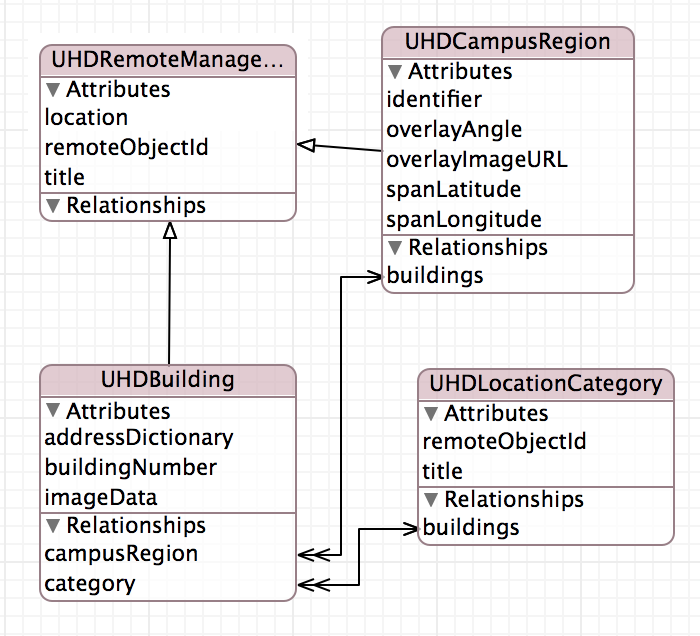
\includegraphics[scale=0.5]{Bilder/DataModel.png}}
\caption{Data Model der Maps}
\end{figure}

Zunächst ist klar, dass Gebäude als eine eigenständige Klasse implementiert werden müssen. Da jedes Gebäude einen Ort zugewiesen bekommt, welcher in der Karte durch eine Annotation eingefügt wird, muss das \objc{MKAnnotation}-\emph{Protokoll} implementiert werden. Annotations haben im Deutschen die Bedeutung \emph{Anmerkung} und erfüllen den Zweck Metadaten in den Quelltext der App zu integrieren, in unserem Fall die Location des Gebäudes. Dies wird für den \objc{UHDMapsViewController} in Abschnitt \ref{subsection_2} wichtig werden, da dort eine \objc{MKMapView} implementiert wird, auf der die gewünschten Gebäude angemerkt werden sollen, also mit einer Annotation versehen werden. Dazu wird nun die Klasse \objc{UHDRemoteManagedLocation} erstellt, welche gerade das\objc{MKAnnotation}-\emph{Protokoll} implementiert. Diese Klasse ordnet jedem Gebäude verschiedene Eigenschaften, wie den Ort, aber auch einen Titel zu. Die Gebäude selbst werden in der Klasse \objc{UHDBuilding} implementiert, welche jedem Gebäude zusätzlich ein Bild, eine \objc{campusRegion} und eine Kategorie aus der später erläuterten Klasse \objc{UHDLocationCategory} zuweist. Weiterhin wird jedem Objekt der Klasse ein \objc{identifier} übergeben, welcher den Titel richtig zusammensetzt. Dieser wird in Bild \ref{bild_1} nicht dargestellt, da er eine unveränderliche Eigenschaft jedes Gebäudes ist. Diese Art der Implementierung ist sinnvoll, da beispielsweise alle Gebäude im Neuenheimer Feld den Zusatz \emph{INF} tragen, sodass dem Gebäude nur eine \objc{buildingNumber} zugeordnet werden muss. Der eigentliche \objc{title} des Gebäudes setzt sich dann aus beiden Teilen zusammen, was aufgrund der überschriebenen Getter-Methode des Identifiers geschieht:

\begin{objclst}
- (NSString *)identifier {
    return [NSString stringWithFormat:@"%@ %@", self.campusRegion.identifier, self.buildingNumber];
}
\end{objclst}

\noindent Um eine solche Charakterisierung der Gebäude durchzuführen, muss jedem Gebäude eine Region in Heidelberg zugeordnet werden, welche um größten Teil dem jeweiligen Campus entspricht. Dafür wird eine weitere Klasse \objc{UHDCampusRegion} erstellt, die es ermöglicht jedem Gebäude eine solche \objc{campusRegion} zuzuordnen. Auch jede \objc{campusRegion} hat einen eigenen Identifier, welcher in der oben beschriebenen Getter-Methode für den Identifier der \objc{UHDBuilding}-\emph{Klasse} zu einem zusammengesetzten String übergeben wird. Damit erhält man also beispielsweise mit dem Identifier \objc{INF} für das Neuenheimer Feld als eine \objc{campusRegion} und einer Gebäudenummer, z.B. \objc{227}, den \objc{building.indetifier} \objc{INF 227}. Im Falle der Altstadt mit dem Identifier \objc{Altstadt} entspricht dieser dem Identifier für das Gebäude selbst. Somit kann der Benutzer zum Beispiel im \objc{UHDBuildingDetailView} direkt sehen, in welchem Bereich von Heidelberg das ausgewählte Gebäude liegt. Durch einen \objc{NSMutableSet} können einer \objc{campusRegion} mehrere Gebäude hinzugefügt werden. Die Klasse \objc{UHDCampusRegion} implementiert zudem das \objc{MKOverlay}-\emph{Protokoll}, welches später für die zusätzliche Kartenansicht in der View interessant wird. Damit kann eigenes Kartenmaterial, wie die Lagekarten der Universität Heidelberg, über die eigentliche Map gelegt werden, um somit die Gebäude der Universität hervorzuheben. Da Objekte der Klasse \objc{UHDCampusRegion} ähnlich wie diejenigen aus \objc{UHDBuilding} einen Ort zugewiesen bekommen, welcher für eine \objc{campusRegion} allerdings dem Mittelpunkt entspricht, werden beide Klassen als Subklassen von \objc{UHDRemoteManagedLocation} implementiert. Um weiterhin zwischen Gebäuden verschiedener Fakultäten oder auch Verwaltungsgebäuden zu unterscheiden, wird eine weitere Klasse \objc{UHDLocationCategory} erstellt, die jedem Objekt der Klasse \objc{UHDBuilding} eine \objc{category} zuordnet. Dadurch kann man beispielsweise im \objc{UHDMapsSearchTableViewController}, welcher in Abschnitt \ref{subsection_1} behandelt wird, speziell nach Gebäuden einer Fakultät suchen oder sich nur Gebäude einer bestimmten Kategorie ansehen. 

\newpage

\section{Darstellung der verschiedenen Views}

\begin{figure}[ht]\label{bild_2}
\centering \rotatebox{0}{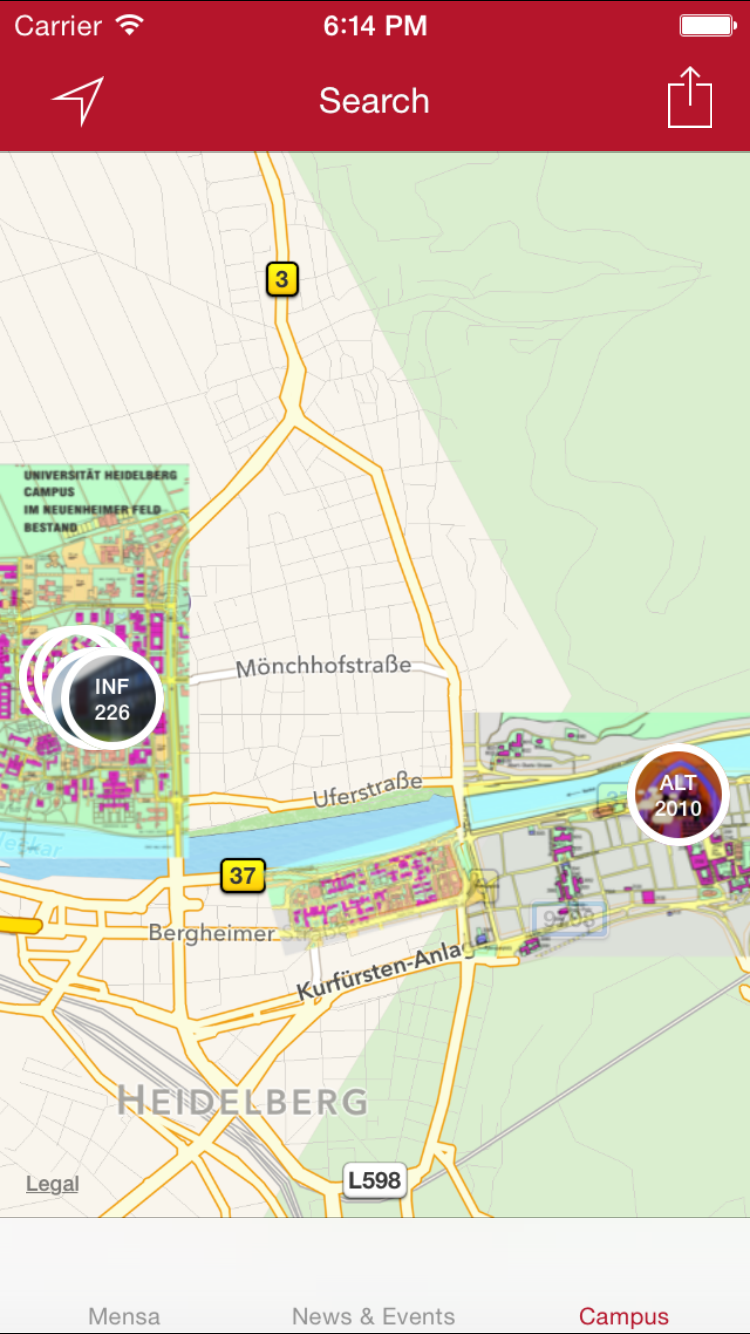
\includegraphics[scale=0.13]{Bilder/Bild_1.png}}
\caption{Ansicht der MapView nach Auswahl des \objc{Campus}-Buttons}
\end{figure}

Im \objc{NavigationViewController} kann über den Button \objc{Campus} die Anzeige der \objc{MKMapView} erreicht werden. Zunächst befindet sich in der oberen linken Ecke ein Button in der Form einer Kompassnadel. Mit Hilfe dieses Buttons kann der Benutzer seine eigene Position anzeigen lassen und durch zweifaches Drücken die Ausrichtung seinen mobilen Geräts bestimmen. In der MapView werden einzelne Gebäude durch sogenannte \emph{Annotations} gekennzeichnet. Diese haben den Zweck bestimmte Orte auf der \objc{mapView} auszuzeichnen. In der Klasse \objc{UHDBuildingAnnotationView} werden die Annotations angepasst, das heißt zum einen wird das Auftreten in der Map View durch ein Symbol und die Darstellung der Annotation selbst, beispielsweise mit Bild des Gebäudes oder einem Info-Button zur Weiterleitung auf den \objc{UHDBuildingDetailViewController}, bearbeitet. Die einzelnen Gebäude der Universität werden durch Symbole dargestellt, was hier zunächst nur provisorisch erstellt wurde. Bisher sind wir uns noch nicht sicher, wie wir jedes einzelne Gebäude markieren können, ohne dass dabei die Übersichtlichkeit verloren geht, wie es im folgenden Bild bereits bei nur $4$ solchen Symbolen der Fall ist. 

\begin{figure}[ht]\label{bild_3}
\centering \rotatebox{0}{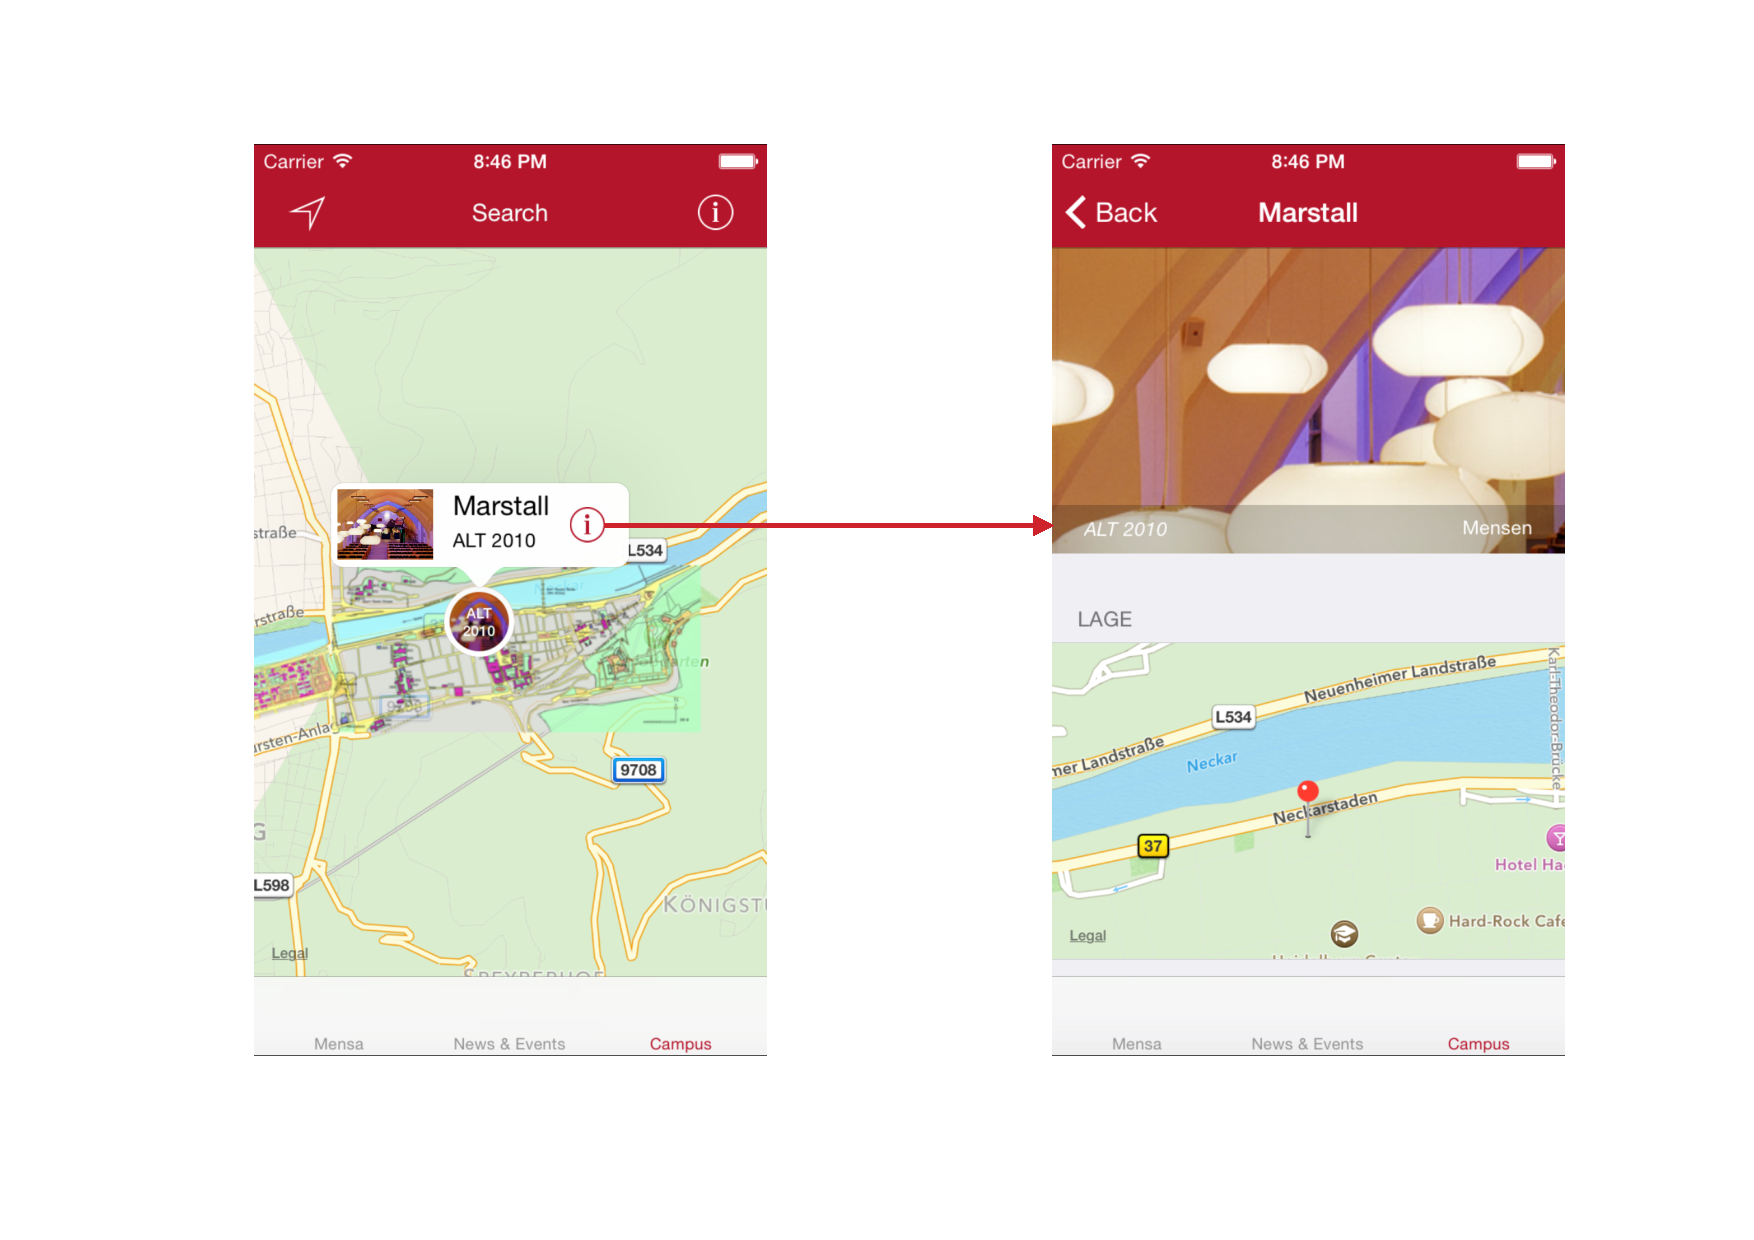
\includegraphics[scale=0.42]{Bilder/Bild_4.png}}
\caption{\objc{AnnotationView} und \objc{UHDBuildingDetailViewController}}
\end{figure}

Durch die Auswahl eines solchen Symbols erhält man zunächst grundlegende Informationen, wie den Titel und die Campus-Zugehörigkeit, in einer Art Sprechblase angezeigt. Das Tappen auf den Info-Button in dieser Sprechblase öffnet ein neues Fenster, welches alle Informationen zum Gebäude anzeigt. Diese Darstellung wird durch den \objc{UHDBuildingDetailViewController} implementiert. Zu den von Apple bereitgestellten Kartenansichten, lässt sich die MapView, wie bereits im vorherigen Kapitel angesprochen, durch ein sogenanntes Overlay modifizieren. Diese Kartendarstellung ist ein wenig aufwendiger zu implementieren, denn diese ist keine von Apple vorgefertigte Anzeige Option. Stattdessen wurde dazu aus verschiedenen Lagekarten der Universität im PNG-Format, welches die Gebäude in verschiedenen Farben und mit Namen anzeigt, benutzt, um ein solches Overlay zu erzeugen. Das heißt über die \objc{MapView} wurde das Bild gelegt, indem dort die Mitte mit der Property \objc{coordinate} sowie Höhe und Breite durch \objc{spanLatitude} und \objc{spanLongitude} (siehe \objc{UHDCampusRegion.m}) festgelegt werden. Durch Bestimmung der Breite \objc{spanLongitude} und der Höhe \objc{spanLatitude} des Bildes in geographischen Koordinaten konnte das \objc{boundingMapRect} konfiguriert werden und dadurch die genaue Position des Overlays eingestellt werden. 

\begin{figure}[ht]\label{bild_4}
\centering \rotatebox{0}{\includegraphics[scale=0.41]{Bilder/Bild_2.1.png}}
\caption{Overlay anhand des Beispiels Neuenheimer Feld}
\end{figure}

Wir haben uns für diese zusätzliche Darstellung entschieden, da sie dem Benutzer einen besseren Überblick über die Gebäude der Universität liefert, als die eigentliche Karte in iOS. Um das Overlay korrekt darzustellen, wurde die Klasse \objc{UHDCampusRegionRender} implementiert, in der das Overlayimage dem View übergeben wird und durch die Methode \objc{- (void)drawMapRect: zoomScale: inContext:} in die jeweilige Region der MapView gelegt wird. Weiterhin haben wir uns gedacht, dass der Nutzer am besten selbst entscheiden sollte, ob er das Overlay benutzen möchte oder nicht. Dazu befindet sich in Bild \ref{bild_4} oben rechts ein Button, durch den ein Slide von unten hineinkommt und dem Benutzer einige Einstellmöglichkeiten bietet. Hierbei wurde ein sogenannter \objc{Switch} eingefügt, mit dem das Overlay ein und ausgeschalten werden kann. Entscheidet sich also der Nutzer dazu, dass er die Map lieber ohne das Overlay benutzen möchte, dann kann er diesen Schalter in der deaktivierenden Position belassen. Bei der Funktionsübersicht gibt es zunächst die Option die Karte in verschiedenen Ansichten darzustellen. Es gibt die Wahl zwischen \objc{Standard}, was die Standarddarstellung der Karte in iOS ist, \objc{Hybrid} oder \objc{Satellit}. Zudem kann jeweils immer zusätzlich das Overlay mit Hilfe des Switch aktiviert beziehungsweise deaktiviert werden. Was wir zu diesem Zeitpunkt noch nicht implementiert haben, ist die Auswahl einzelner Gebäudekategorien. Dies wird später besonders der Übersichtlichkeit dienen, falls man beispielsweise nur Gebäude einer Fakultät suchen möchte.

\begin{figure}[ht]\label{bild_5}
\centering \rotatebox{0}{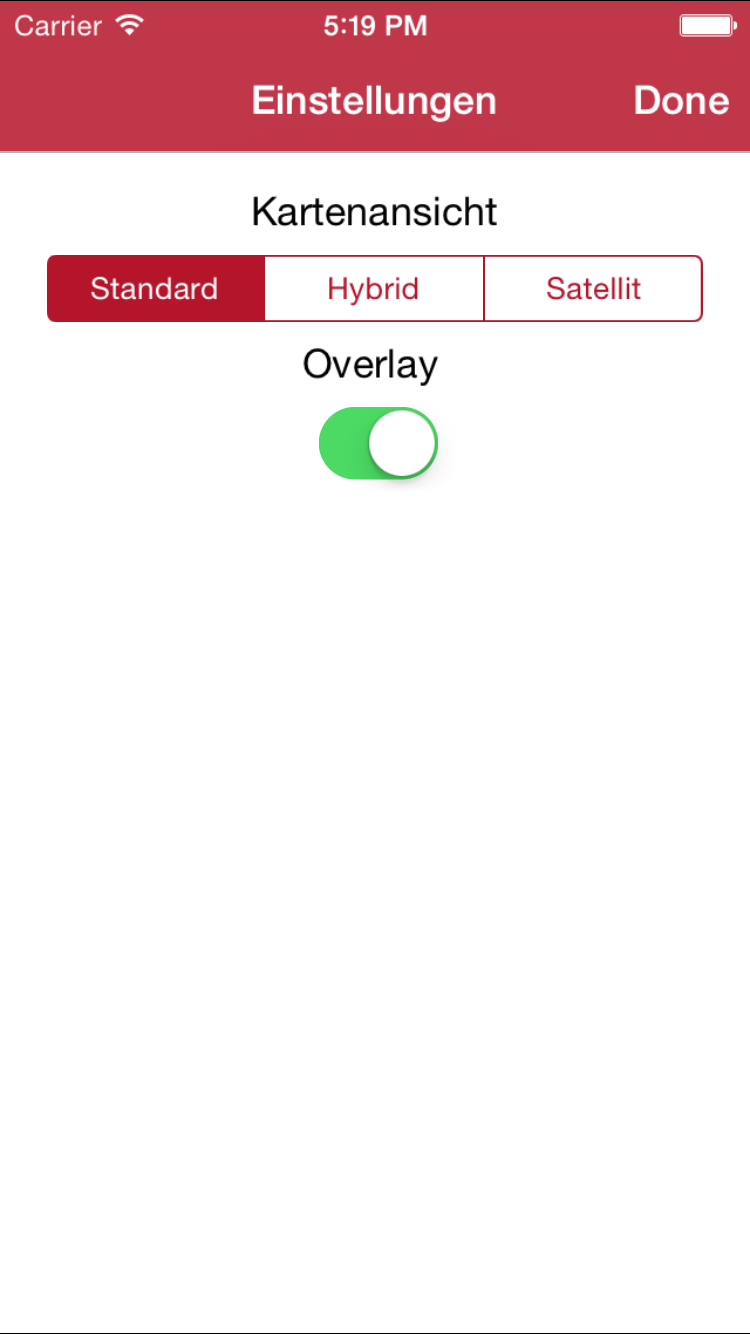
\includegraphics[scale=0.15]{Bilder/Bild_3.png}}
\caption{Vorläufige Dartsellung der Funktionsübersicht}
\end{figure}

Die Funktionsübersicht sieht zugegebenermaßen noch etwas spartanisch aus. Allerdings wollten wir zunächst die Funktionen und die wichtigen Ansichten, wie etwa die \objc{mapView}, implementieren und später alles genauer überarbeiten. Drückt man in Bild \ref{bild_5} auf den mittleren Button mit dem Titel \emph{Search}, so kommt man zunächst zum \objc{UHDMapsSearchTableViewController}, in dem einzelne Gebäude nach Kategorien geordnet dargestellt werden.

\begin{figure}[ht]\label{bild_6}
\centering \rotatebox{0}{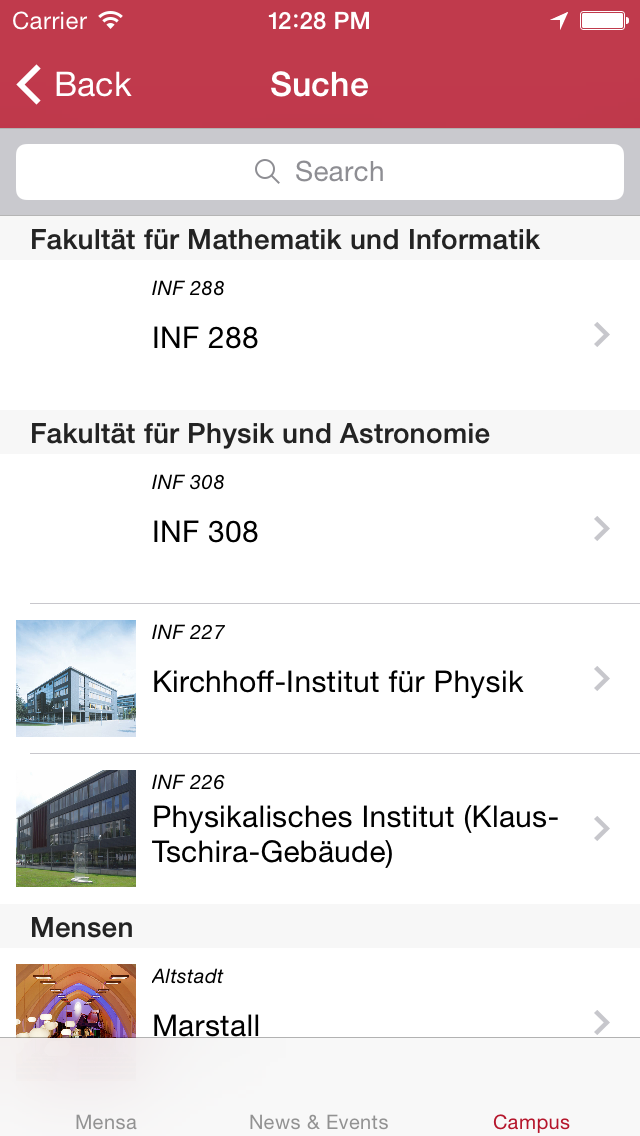
\includegraphics[scale=0.15]{Bilder/Bild_5.png}}
\caption{\objc{UHDMapsSearchTableViewController} mit Beispiel Daten}
\end{figure}

Dort wurde mit Hilfe einer \objc{UISearchBar} eine Suchfunktion integriert, bei dem nach bestimmten Gebäuden oder auch Gebäuden einer Fakultät gesucht werden kann. Zudem wurde die \objc{UITableView} in \objc{sections} unterteilt, welche die Gebäude einer Kategorie zusammenfasst. Mit einem Tap auf das gewünschte Gebäude kommt man auf die \objc{UHDBuildingDetailView}, wie sie in Bild \ref{bild_3} zu sehen ist. Dort sind alle Informationen über das Gebäude zusammengefasst dargestellt. Hier wird es vermutlich noch zu Erweiterungen hinsichtlich der angezeigten Daten kommen. Wir planen zudem Räume innerhalb der Gebäude, Professoren und Forschungsgruppen am jeweiligen Gebäude aufzulisten.

\section{Implementierung der View Controller}

\subsection{UHDMapsViewController}\label{subsection_2}

In diesem View Controller werden die Methoden im ersten View implementiert. Dabei enthält die Map View alle Gebäude der Universität und kennzeichnet diese mit einer Annotation. Dazu muss eine Datenbankabfrage mit Hilfe eines \objc{NSFetchedResultsController} durchgeführt werden. Die zugehörige Methode wurde folgendermaßen implementiert:

\begin{objclst}
- (NSFetchedResultsController *)fetchedResultsController {
    if (!_fetchedResultsController) {
        NSFetchRequest *fetchRequest = [NSFetchRequest fetchRequestWithEntityName:[UHDBuilding entityName]];
        fetchRequest.sortDescriptors = @[[NSSortDescriptor sortDescriptorWithKey:@"title" ascending:YES]];
        NSFetchedResultsController *fetchedResultsController = [[NSFetchedResultsController alloc] initWithFetchRequest:fetchRequest managedObjectContext:self.managedObjectContext sectionNameKeyPath:nil cacheName:nil];
        fetchedResultsController.delegate = self;
        [fetchedResultsController performFetch:NULL];
        self.fetchedResultsController = fetchedResultsController;
    }
    return _fetchedResultsController;
}
\end{objclst}

Zunächst wird in Zeile $3$ eine \objc{NSFetchRequest} durchgeführt, welche auf die Klasse \objc{UHDBuilding} zugreift. Mit Hilfe des \objc{fetchedRequest.sortDescriptors} werden die einzelnen Gebäude sortiert, wobei hier mit der Methode \objc{sortDescriptorWithKey:@"title" ascending:YES} die Sortierung alphabetisch nach dem Titel durchgeführt wird. Hier können zusätzliche weitere Sortierungen durchgeführt werden, beispielsweise zunächst nach den verschiedenen Kategorien der Gebäude und innerhalb dieser Gruppen wiederum alphabetisch nach dem Titel eines Gebäudes. Als nächstes wird in Zeile $5$ ein \objc{NSFetchedResultsController} erstellt, welcher mit der zuvor erstellten \objc{fetchedRequest} und dem \objc{managedObjectContext} aus \objc{UHDMapsViewController.h} erstellt wird. In Zeile $6$ wird das \objc{Delegate} des \objc{fetchedResultsController} auf \objc{self} gesetzt, da dieses in \objc{UHDMapsViewController.m} deklariert wird. In der nächsten Zeile wird die Datenbankabfrage durchgeführt und abschließend der erstellte \objc{fetchedResultsController} übergeben. Nun verfügt der View Controller über alle nötigen Informationen der Gebäude. Eine ähnliche Abfrage wird ebenfalls für die Objekte der Klasse \objc{UHDCampusRegion} gemacht, um die Overlays an den richtigen Stellen darzustellen. In der Datei \objc{UHDMapsViewController.m} wird ebenfalls das \objc{MKMapViewDelegate} deklariert, so dass hier mit der Methode \objc{(MKAnnotationView *)mapView:(MKMapView *)mapView viewForAnnotation:(id <MKAnnotation>)annotation} die Annotations aufgerufen werden.

\begin{objclst}
- (MKAnnotationView *)mapView:(MKMapView *)mapView viewForAnnotation:(id <MKAnnotation>)annotation {
    UHDBuilding *building = (UHDBuilding *)annotation;
    NSArray *allBuildings = self.fetchedResultsController.fetchedObjects;    
    if ([allBuildings containsObject:building]) {
        static NSString *buildingAnnotationViewIdentifier = @"buildingAnnotation";
        UHDBuildingAnnotationView *buildingAnnotationView = (UHDBuildingAnnotationView *)[mapView dequeueReusableAnnotationViewWithIdentifier:buildingAnnotationViewIdentifier];
        if (!buildingAnnotationView) {
            buildingAnnotationView = [[UHDBuildingAnnotationView alloc] initWithAnnotation:building reuseIdentifier:buildingAnnotationViewIdentifier];
            buildingAnnotationView.canShowCallout = YES;
        } else {
            buildingAnnotationView.annotation = building; 
       	}        
        return buildingAnnotationView;
    }
    return nil;
}
\end{objclst}

Zunächst wird in Zeile $2$ ein Objekt der Klasse \objc{UHDBuilding} als \objc{annotaion} aufgerufen. In Zeile $3$ wird ein \objc{NSArray} mit allen verfügbaren Gebäuden erstellt, das der darauffolgenden \objc{if}-Abfrage dient. Daraufhin wird in Zeile $6$ ein Objekt \objc{buildingAnnotationView} erstellt, welches aus der Klasse \objc{UHDBuildingAnnotationView} stammt und bereits im vorangegangenen Kapitel erstellt wurde. In Zeile $8$ wird schließlich die \objc{buildingAnnotationView} konfiguriert und ihr das zugehörige \objc{building} übergeben. 

\subsection{UHDMapsSearchTableViewController} \label{subsection_1}

In diesem Abschnitt soll genauer auf die Option der Suche nach Gebäuden eingegangen werden. Zunächst wird die Methoder \objc{(BOOL)searchDisplayController:(UISearchDisplayController *)Controller shouldReloadTableForSearchString:(NSString *)searchString} implementiert, welche die gefilterten Objekte bestimmt. 

\begin{objclst}
#pragma mark - Search Results Filtering

-(BOOL)searchDisplayController:(UISearchDisplayController *)Controller shouldReloadTableForSearchString:(NSString *)searchString
{    
    self.filteredObjects = [self.fetchedResultsControllerDataSource.fetchedResultsController.fetchedObjects filteredArrayUsingPredicate:[NSPredicate predicateWithFormat:@"title CONTAINS[cd] %@", searchString]];
    return YES;
}
\end{objclst}

Dazu erhält der \objc{UHDMapsSearchTableViewController} eine \objc{property} der Form \objc{NSArray *filteredObjects}. In der oben aufgeführten Methode wird dieses Array mit Objekten gefüllt, die eine bestimmte Bedingung erfüllen. Es wird eine Datenbankabfrage durchgeführt, welche mit einem \objc{NSPredicate} die gesuchten Objekte klassifiziert. In diesem Fall tippt der Benutzer ein Suchwort oder auch nur Buchstaben in die \objc{UISearchBar} ein, die im Titel des gewünschten Objektes stecken. Aus diesem Grund wird durch \objc{[NSPredicate predicateWithFormat:@"title CONTAINS[cd] \%@", searchString]} bei der Abfrage überprüft, ob der Titel eines Objekts die gesuchten Wörter enthält. Dabei ist \objc{searchString} der Zugriff auf den eingegebenen String in die \objc{UISearchBar}. Mit \objc{CONTAINS} wird angegeben, was das gesuchte Objekt erfüllen soll, nämlich dass die eingegebene Zeichenkette im Titel enthalten ist, und durch den Suffix \objc{[cd]} wird die Suche unabhängig von Groß- bzw. Kleinschreibung und diakritischen Zeichen, wie Umlaute oder Buchstaben mit Akzenten. Nun wurden die Suchfunktion als solche implementiert. Um jeweils die richtigen Objekte in der \objc{TableView} anzuzeigen, ist folgender Code nötig:

\begin{objclst}
- (UITableViewCell *)tableView:(UITableView *)tableView cellForRowAtIndexPath:(NSIndexPath *)indexPath
{
	UITableViewCell *cell;
    UHDBuilding *item;
    if (tableView==self.searchDisplayController.searchResultsTableView) {
        cell = [self.tableView dequeueReusableCellWithIdentifier:@"mapsSearchCell"];
        item = [self.filteredObjects objectAtIndex:indexPath.row];
    } else {
		cell = [self.tableView dequeueReusableCellWithIdentifier:@"mapsSearchCell" forIndexPath:indexPath];
		item = [self.fetchedResultsControllerDataSource.fetchedResultsController objectAtIndexPath:indexPath];
    }
    [(UHDMapsSearchCell *)cell configureForItem:item];
	return cell;
}
\end{objclst}

Hierbei wird unterschieden, ob der Benutzer bestimme Objekte durch Eingabe eines Strings in die \objc{searchBar} sucht oder nur die gesamte Liste benutzt. Dabei wird in Zeile $5$ mit einer \objc{if}-Abfrage überprüft, ob gerade die \objc{searchDisplayController.searchResultTableView} der eigentlichen \objc{TableView} zugewiesen wird. Dann werden mit Hilfe der Zeilen $6$ und $7$ die Zellen mit dem Identifier \objc{@"mapsSearchCell"} eingefügt und jeweils mit einem Item aus dem Array \objc{filteredObjects} versehen. Ist dies nicht der Fall, so werden der \objc{TableView} gerade alle Objekte zugewiesen, indem auf den \objc{fetchedResultsController} zugeriffen wird. Zum Schluss muss noch gewährleistet werden, dass bei der Auswahl eines bestimmten Gebäudes die richtigen Informationen in einem neuen \objc{ViewController} dargestellt werden. Dazu dient der folgende Abschnitt:

\begin{objclst}
- (void)prepareForSegue:(UIStoryboardSegue *)segue sender:(id)sender
{
    if ([segue.identifier isEqualToString:@"showBuildingDetail"])
    {
        UHDBuildingDetailViewController *destViewController = segue.destinationViewController;
        if (self.searchDisplayController.active)
        {
            NSIndexPath *indexPath= nil;
            UHDBuilding *item = nil;
            indexPath = [self.searchDisplayController.searchResultsTableView indexPathForSelectedRow];
            item = [self.filteredObjects objectAtIndex:indexPath.row];
            destViewController.building = item;
        } else
        {
            destViewController.building = [self.fetchedResultsControllerDataSource.fetchedResultsController objectAtIndexPath:[self.tableView indexPathForCell:(UITableViewCell *)sender]];
        }
    }
}
\end{objclst}

Dabei besteht nur die Schwierigkeit, dass bei einer durchgeführten Suche nicht mehr die Gebäude wie zuvor nach Kategorie und Namen sortiert sind. Deshalb muss sichergestellt werden, dass das richtige Objekt übergeben wird. Dies geschieht in den Zeilen $6$ bis $13$, wobei durch einen Zugriff auf die \objc{searchResultsTableView} die ausgewählte Zelle bestimmt wird. Aus dieser Zelle wird dann also das Objekt genommen und an den \objc{destViewController}, welcher in diesem Falle der \objc{UHDBuildingDetailViewController} ist, übergeben. Damit erhält man also die Ansicht aus Bild \ref{bild_3}.

\newpage
\chapter{Zusammenfassung}

Im letzten Abschnitt wurden nur einzelne Code-Stücke beispielhaft aufgeführt, um verschiedene Methoden in den View Controllern zu beschreiben. Dabei wurde nicht jeder einzelne Implementierungsabschnitt oder ViewController aufgeführt, da dies bei weitem zu umfangreich geworden wäre. Zum Zeitpunkt dieser Dokumentation haben wir einige neue Ideen aufgegriffen, die zu weiteren Veränderungen zur bisherigen Darstellung führen. Wie bereits angemerkt wird die View die Einstellungen der \objc{mapView} betreffend noch überarbeitet und vollständig implementiert. Das heißt wir werden Optionen, wie das Filtern nach bestimmten Kategorien von Objekten, ermöglichen. Weiterhin wird der bisherige \objc{Search}-Button in der Mitte der Navigation Bar entfernt und durch eine Suchleiste ersetzt, damit der Benutzer direkt auf der Startseite nach bestimmten Gebäuden suchen kann. Das wichtigste ist jedoch die optimale Benutzeroberfläche für die \objc{mapView} zu finden, denn einerseits sollen die gewünschten Regionen eindeutig erkennbar sein, aber andererseits sollen dadurch nicht andere Abschnitte überdeckt werden, wie es derzeit durch die runden Symbole der Fall ist. Zuvor hatten wir die üblichen Pins verwendet, was allerdings auch zu einer unübersichtlichen Darstellung führt. Eine zusätzliche Möglichkeit, die wir derzeit in Betracht ziehen, ist das Splitten des Overlays in die verschiedenen Gebäude, so dass jedes Objekt der Klasse \objc{UHDBuilding} eine Region der Grundfläche entsprechend zugewiesen bekommt. Dann könnte Beispielsweise bei der Suche nach einem solchen Gebäude dessen Overlay angezeigt werden, was sich schließlich von allen anderen Gebäuden abhebt. Wir haben noch einiges an Arbeit vor uns, allerdings erkennt man eindeutig die erzielten Ergebnisse. Ich habe jedenfalls große Fortschritte im Programmieren unter Objective-C gemacht und freue mich auch weiterhin am diesem Projekt teilzunehmen.



\end{document}